\documentclass[11pt]{beamer}
\usetheme{Boadilla}
\usecolortheme{seahorse}
\usepackage[utf8]{inputenc}
\usepackage[spanish]{babel}
\usepackage{amsmath}
\usepackage{amsfonts}
\usepackage{amssymb}
\usepackage{graphicx}
\usepackage{algorithm}
\usepackage[]{algpseudocode}
\usepackage{varwidth}
\usepackage{float}

\floatname{algorithm}{Algoritmo}
\algrenewcommand\algorithmicrequire{\textbf{Requiere}}
\algrenewcommand\algorithmicfor{\textbf{Para}}
\algrenewcommand\algorithmicdo{\textbf{hacer}}
\algrenewcommand\algorithmicif{\textbf{si}}
\algrenewcommand\algorithmicthen{\textbf{entonces}}
\algrenewcommand\algorithmicelse{\textbf{sino}}
\algrenewcommand\algorithmicreturn{\textbf{Retornar}}
\algrenewcommand\algorithmicend{\textbf{Fin}}
\algrenewcommand\algorithmicfunction{\textbf{Función}}
\algrenewcommand\algorithmicprocedure{\textbf{Procedimiento}}
\algrenewcommand\alglinenumber[1]{\tiny #1:}

\DeclareMathOperator*{\argmin}{argmin}
\DeclareMathOperator*{\argmax}{argmax}

\author[Carolina Higuera Arias]{Carolina Higuera Arias\\ \bigskip \textit{Asesor:} Ph.D Fernando Enrique Lozano Martinez}
\title[Control de tránsito con MARL]{Control de intersecciones semaforizadas aplicando aprendizaje por refuerzo multiagente}
\institute[Uniandes] 
{
Universidad de los Andes \\ 
\medskip
}
\titlegraphic{
\includegraphics[scale=0.5]{./graficas/uniandes.eps}}
\date{Diciembre 16, 2016}

\begin{document}


\section{A1: Q-VE}
\begin{frame}
\frametitle{Q-Learning con grafos de coordinación}

%\begin{algorithm}[H]
%\tiny %\small, \footnotesize, \scriptsize, or \tiny
%\caption{\tiny Q-Learning multiagente con grafos de coordinación}\label{alg:Q-VE}
\scriptsize
\begin{algorithmic}[1]
\Require grafo de coordinación del sistema $G=(\mathcal{V},\mathcal{E})$; orden de eliminación de los agentes $\mathcal{O}\subseteq \mathcal{V}$; conjunto de vecinos para cada agente $\Gamma(i)$
\For{cada arco $(i,j) \in \mathcal{E}$}
	\State Inicialice $Q_{ij}(s_{ij},a_i,a_j)$ de manera optimista
\EndFor
\For{cada episodio}
	\State Inicialice el estado observado $s_i$ para todos los agentes $i \in \mathcal{V}$
	\For{cada periodo de decisión $k$}
		\State Obtenga la acción conjunta $\mathbf{a}$ con $\epsilon-$greedy como método de selección 
		\State Para cada agente $i \in \mathcal{V}$: aplique $a_i \in \mathbf{a}$, observe $r_i$ y $s_i^k$
		\State Para todos los arcos $(i,j) \in \mathcal{E}$: forme $s_{ij}^k=s_i^k \cup s_j^k$
		\State Obtener $\mathbf{a}^*=\max_{\mathbf{a}}Q(\mathbf{s^k},\mathbf{a}) \rightarrow$ \Call{EliminaciónVariable}{$s_{ij}^k \forall (i,j)\in \mathcal{E}$}
		\For{cada arco $(i,j) \in \mathcal{E}$}
			\State \tiny $Q_{ij}(s_{ij}^{k-1},a_i^{k-1},a_j^{k-1}):= (1-\alpha)Q_{ij}(s_{ij}^{k-1},a_i^{k-1},a_j^{k-1})+ \alpha \left[ \frac{r_i^k}{|\Gamma(i)|}+\frac{r_j^k}{|\Gamma(j)|}+ \gamma Q_{ij}(s_{ij}^k,a_i^*,a_j^*) {\vphantom{\frac{r_i}{|\Gamma(i)|}}} \right]$ \scriptsize
		\EndFor
		\State Para cada agente $i \in \mathcal{V}$ actualice $s_i^{k-1} \leftarrow s_i^k$
	\EndFor
\EndFor
\end{algorithmic}
%\end{algorithm}
\end{frame}

\section{A2: VE}
\begin{frame}
\frametitle{Algoritmo de eliminación de variable}
\tiny
\begin{algorithmic}[1]
\Function{EliminaciónVariable}{$s_{ij}^k$}
\For{cada agente $i \in \mathcal{O}$}
	\State Calcular función de pago condicional $\phi$
	\If{el agente $i$ es el primero a eliminar}
		\State $k \equiv $siguiente agente a eliminar, $k\in \Gamma(i)$
		\State $\phi_{kj}=\max_{a_i}\left[\sum_{j \in \Gamma(i)}Q_{ij}(s_{ij}^k,a_i,a_j)\right]$
	\ElsIf{el agente $i$ es el último a eliminar}
		\State $\phi_i=\max_{a_i}[\phi_i(a_i)]$	
	\Else
		\State $k \equiv $siguiente agente a eliminar, $k\in \Gamma(i)$
		\State $\phi_{kj}=\max_{a_i}\left[\sum_{j \in \Gamma(i)}Q_{ij}(s_{ij}^k,a_i,a_j)+\phi_{ik}(a_i,a_k)\right]$
	\EndIf
	\State Transmitir $\phi$ al siguiente agente a eliminar
\EndFor
\Statex
\For{cada agente $i$ en el orden inverso de $\mathcal{O}$}
	\If{el agente $i$ fue el último eliminado}
		\State Obtener $a_i^*=\argmax_{a_i}[\phi_i(a_i)]$
		\State Transmitir al agente anterior $a_i^*$
		\State Transmitir $\max_{\mathbf{a}}Q(\mathbf{s},\mathbf{a})=\max_{a_i}\phi_i(a_i)$
	\Else
		\State Esperar de los agentes vecinos $a_k^*$, $a_j^*$ y $\max_{\mathbf{a}}Q(\mathbf{s},\mathbf{a})$
		\State Obtener $a_i^*=\argmax_{a_i}[\phi_{kj}(a_k^*,a_j^*)]$
	\EndIf
\EndFor
\State \Return $a_i^* \quad \forall \quad i \in \mathcal{V}$
\EndFunction
\end{algorithmic}
\end{frame}

\section{A3: Q-BR}
\begin{frame}
\frametitle{Q-Learning con \textit{best response}}
\tiny
\begin{algorithmic}[1]
\Require conjunto de agentes $N$, conjunto de vecinos para cada agente $\mathrm{NB}_i$
\For{cada agente $i \in \{1,2,\cdots,|N|\}$}
	\For{cada agente vecino $j \in \{1,2,\cdots,|\mathrm{NB}_i|\}$}
		\State Inicializar $Q_{i,\mathrm{NB}_i[j]}(s_{i,\mathrm{NB}_i[j]},a_i,a_{\mathrm{NB}_i[j]})$ de manera optimista
		\State Inicializar modelo para la estimación de política $\theta_{i,\mathrm{NB}_i[j]}(s_{i,\mathrm{NB}_i[j]},a_{\mathrm{NB}_i[j]})=1/|\mathcal{A}_{\mathrm{NB}_i[j]}|$
	\EndFor
\EndFor
\Statex
\For{cada episodio}
	\State Inicializar el estado observado $s_i$ para todos los agentes $i \in N$
	\For{cada periodo de decisión $k$}
		\State Obtener la acción conjunta $\mathbf{a}$ con $\epsilon-$greedy como método de selección

		\State Aplicar $a_i \in \mathbf{a}$ para cada agente $i \in \mathcal{V}$
		\For{cada agente $i \in \{1,2,\cdots,|N|\}$}
			\For{cada agente vecino $j \in \{1,2,\cdots,|\mathrm{NB}_i|\}$}
				\State Observar $s_i^k$, $r_i^k$, $s_{\mathrm{NB}_i[j]}^k$ y $a_{\mathrm{NB}_i[j]}^{k-1}$
				\Statex
				\State Formar estado conjunto $s_{i,\mathrm{NB}_i[j]}^k=s_i^k \cup s_{\mathrm{NB}_i[j]}^k$ y acción conjunta $a_{i,\mathrm{NB}_i[j]}^{k-1}=a_i^{k-1} \cup a_{\mathrm{NB}_i[j]}^{k-1}$
				\Statex
				\State \begin{varwidth}[t]{\linewidth} Actualizar modelo de estimación de la política para el vecino $\mathrm{NB}_i[j]$: \par \hskip\algorithmicindent $\theta_{i,\mathrm{NB}_i[j]}(s_{i,\mathrm{NB}_i[j]}^{k-1}, a_{\mathrm{NB}_i[j]}^{k-1})=\frac{v(s_{i,\mathrm{NB}_i[j]}^{k-1}, a_{\mathrm{NB}_i[j]}^{k-1})}{\sum_{a_{\mathrm{NB}_i[j]} \in \mathcal{A}_{\mathrm{NB}_i[j]}} v(s_{i,\mathrm{NB}_i[j]}^{k-1}, a_{\mathrm{NB}_i[j]})}$ \end{varwidth}
				\Statex
				\State \begin{varwidth}[t]{\linewidth} Encontrar la \textit{best response} respecto al vecino $\mathrm{NB}_i[j]$: \par \hskip\algorithmicindent $\begin{aligned} br_i^k=\max_{a_i \in \mathcal{A}_i} \left[ \sum_{a_{\mathrm{NB}_i[j]} \in \mathcal{A}_{\mathrm{NB}_i[j]}}  Q_{i,\mathrm{NB}_i[j]}(s_{i,\mathrm{NB}_i[j]}^k,a_{i,\mathrm{NB}_i[j]}) \times  \theta_{i,\mathrm{NB}_i[j]}(s_{i,\mathrm{NB}_i[j]}^k,a_{\mathrm{NB}_i[j]}) {\vphantom{\sum_{a_{NB_i[j]} \in \mathcal{A}_{NB_i[j]}}}} \right] \end{aligned}$ \end{varwidth}
				\Statex
				\algstore{myalg}
\end{algorithmic}
\end{frame}

\begin{frame}
\tiny
\begin{algorithmic}[1]
\algrestore{myalg}
				\State \begin{varwidth}[t]{\linewidth} Actualizar factores $Q$:\par \hskip\algorithmicindent  $\begin{aligned} Q_{i,\mathrm{NB}_i[j]}^k(s_{i,\mathrm{NB}_i[j]}^{k-1},a_{i,\mathrm{NB}_i[j]}^{k-1})=  (1-\alpha)Q_{i,\mathrm{NB}_i[j]}^{k-1} (s_{i,\mathrm{NB}_i[j]}^{k-1},a_{i,\mathrm{NB}_i[j]}^{k-1}) + \alpha \left[ r_i^k+\gamma br_i^k \right] \end{aligned}$ \end{varwidth}
				\Statex
				\State Actualizar $s_{i,\mathrm{NB}_i[j]}^{k-1} \leftarrow s_{i,\mathrm{NB}_i[j]}^k$
			\EndFor
			\Statex
			\State \begin{varwidth}[t]{\linewidth} Acción que corresponde a \textit{best response} con todos  los vecinos: \par \hskip\algorithmicindent  $\begin{aligned} a_i^k=\argmax_{a_i \in \mathcal{A}_i}&\left[ \sum_{j \in \{1,2,\cdots,|\mathrm{NB}_i|\}} \sum_{a_{\mathrm{NB}_i[j]}\in \mathcal{A}_{\mathrm{NB}_i[j]}} \right.\\ & \left. Q_{i,\mathrm{NB}_i[j]}(s_{i,\mathrm{NB}_i[j]}^k,[a_i \cup a_{\mathrm{NB}_i[j]}])  \times \theta_{i,\mathrm{NB}_i[j]}(s_{i,\mathrm{NB}_i[j]}^k,a_{\mathrm{NB}_i[j]}) {\vphantom{\sum_{j \in \{1,2,\cdots,|\mathrm{NB}_i|\}}}} \right] \end{aligned}$ \end{varwidth}			
		\EndFor
	\EndFor
\EndFor
\end{algorithmic}
\end{frame}

\section{A4:VQ}
\begin{frame}
\frametitle{Discretización del espacio de estados}
\tiny
\begin{algorithmic}[1]
\Procedure{Vector Quantization}{}
\For{cada hora $h \in {0,1,\cdots,23}$} 
	\For{cada fase $k$} 
		\State Observar pasivamente el sistema durante $n$ días
		\Statex
		\State \begin{varwidth}[t]{\linewidth} Guardar todos los vectores estado $s \in \mathbb{R}^{2(2+2i)-1}$ y concatenar las $n$ observaciones en una matriz $\mathcal{S}$, \par \hskip\algorithmicindent donde cada columna $j$ represente una dimensión del estado \end{varwidth}	
		\Statex
		\State Calcular la desviación estándar de cada columna $\mathbf{Stdev}(\mathcal{S})_j$
		\Statex
		\State Calcular el número de centroides $C_{h,k}=\sum_j \mathbf{Stdev}(\mathcal{S})_j$
		\Statex
		\State Aplicar K-Means sobre $\mathcal{S}$ usando el número de centroides calculado $\rightarrow \mathrm{VQ}_{h,k}(\mathcal{S})$
	\EndFor
\EndFor
\EndProcedure
\Statex
\Procedure{Discretización}{ estado continuo $s_{ij}$ }
\State \Return $\argmin_{y \in \mathrm{VQ}_{h,k}(s_{ij})}\{d_E(s_{ij},y)\}$
\Comment{ euclidiana }
\EndProcedure
\end{algorithmic}
\end{frame}

\section{A5:fases}
\begin{frame}
\frametitle{Ejemplo de un plan de fases}
\only<1>{
\begin{center}
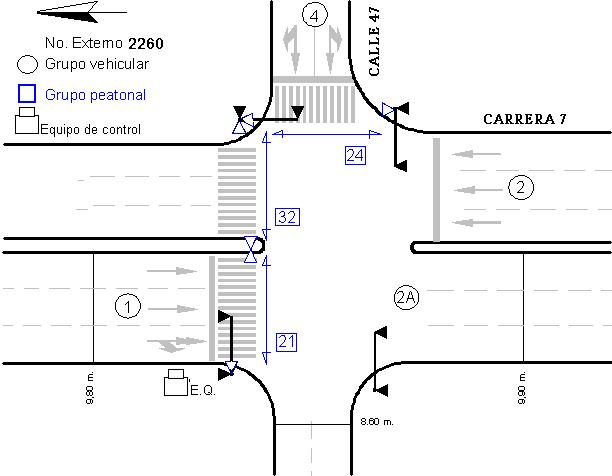
\includegraphics[scale=0.7]{./graficas/ak7cl45.png}
\end{center}}
\pause
\only<2>{
\begin{center}
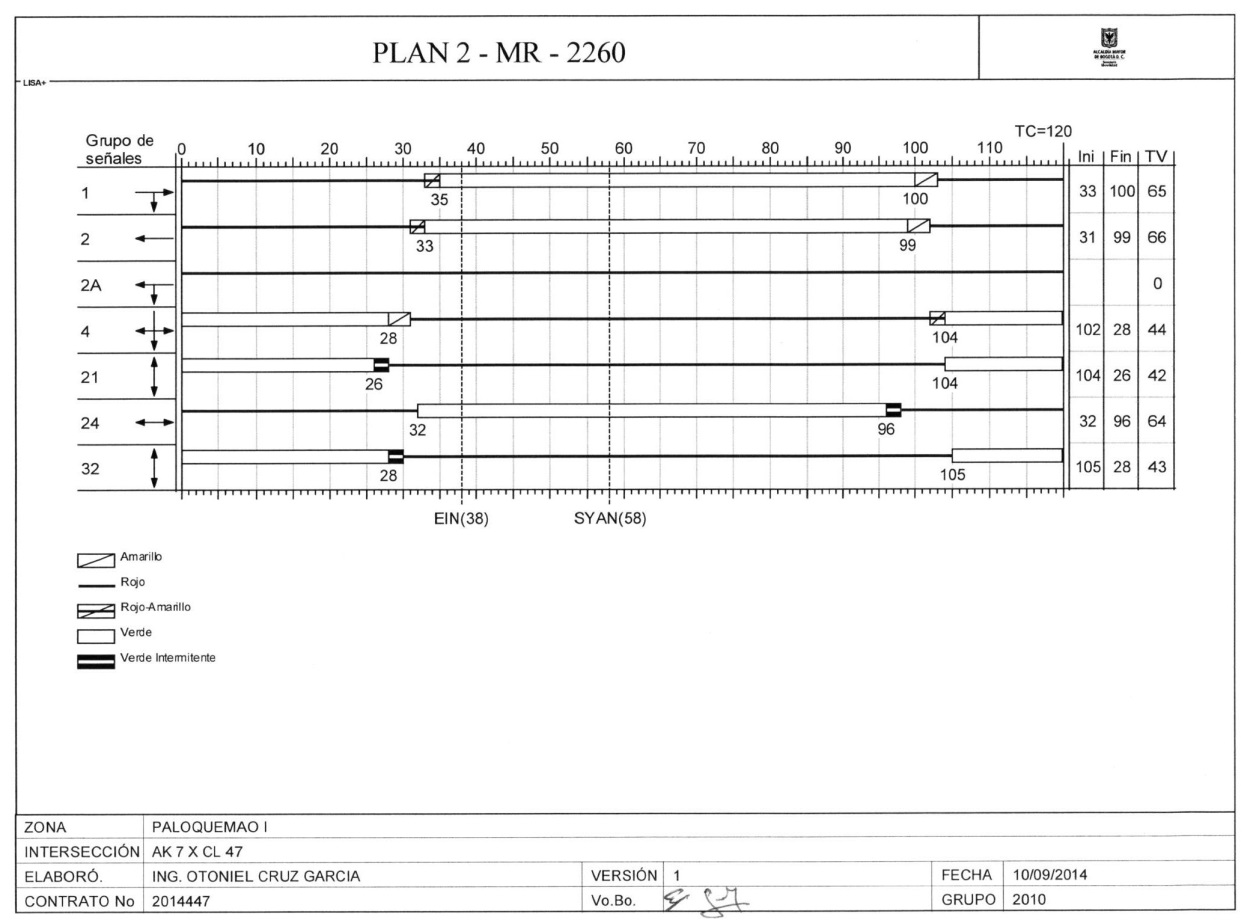
\includegraphics[scale=0.7]{./graficas/plan2.jpg}
\end{center}}
\end{frame}

\section{A6:CO-RL}
\begin{frame}
\frametitle{De control óptimo a aprendizaje por refuerzo}
\only<1>{
La política $\pi$ corresponde a un conjunto de funciones $\pi=\{\mu_0,\mu_1,\cdots\}$ en donde cada $\mu_k$ mapea el estado $s_k$ en una acción de control $a_k=\mu_k(s_k)$, tal que $\mu_k \in A(s_k)$ para todo $s_k$.\\
\bigskip
Costo de seguir la política $\pi$:
$$ J_\pi(s)=\lim_{N\rightarrow \infty} \mathbf{E}\left[\sum_{k=0}^{N}\gamma^k r(s_k,\mu_k(s_k),s_{k+1})|s=s_0\right] $$
\\ \bigskip
La política óptima $\pi^* \in \Pi$ corresponde a aquella que maximiza el funcional:
$$ J_\pi^*(s_0)=\max_{\pi \in \Pi} J_\pi(s_0) $$
}
\pause
\only<2>{
Solucionar la ecuación de Bellman para encontrar el valor óptimo del funcional para una iteración del problema:
$$J_\pi^*(s_i)=\max_{a \in A(s_i)} \sum_{j=1}^{n} p_{s_i,s_j}(a) \left(r(s_i,a,s_j)+\gamma J(s_j)\right), \quad i=1\cdots n$$
\\ \bigskip
D. Bertsekas muestra que se puede obtener el funcional a partir de factores Q óptimos:
$$ Q^*(s_i,a) = \sum_{j=1}^{n} p_{s_i,s_j}(a) \left(r(s_i,a,s_j)+\gamma J^*(s_j)\right), \quad \forall \, (s_i,a)$$
}
\pause
\only<3>{
Reemplazando $J^*(s_i) =\max_{a \in A(s_i)} Q^*(s_i,a)$, se obtiene una ecuación de Bellman para sistemas de estados aumentados:
$$Q^*(s_i,a) = \sum_{j=1}^{n} p_{s_i,s_j}(a) \left(r(s_i,a,s_j)+\gamma \max_{a' \in A(s_j)}Q^*(s_j,a')\right), \quad \forall \, (s_i,a)$$
\\ \bigskip
Una vez calculados los $Q^*(s_i,a) \, \forall \, (s_i,a)$, es directo obtener la política óptima $\pi^*$:
$$\mu^*(s_i)=\argmax_{a\in A(s_i)} Q^*(s_i,a) \quad \forall \, s_i$$
}
\end{frame}

\section{A7:estArte}
%----------D6: estado del arte ------------------
\begin{frame}
\frametitle{Aportes al control de tránsito mediante MARL}
\framesubtitle{Estado del arte: métodos de coordinación (MC)}
\begin{center}
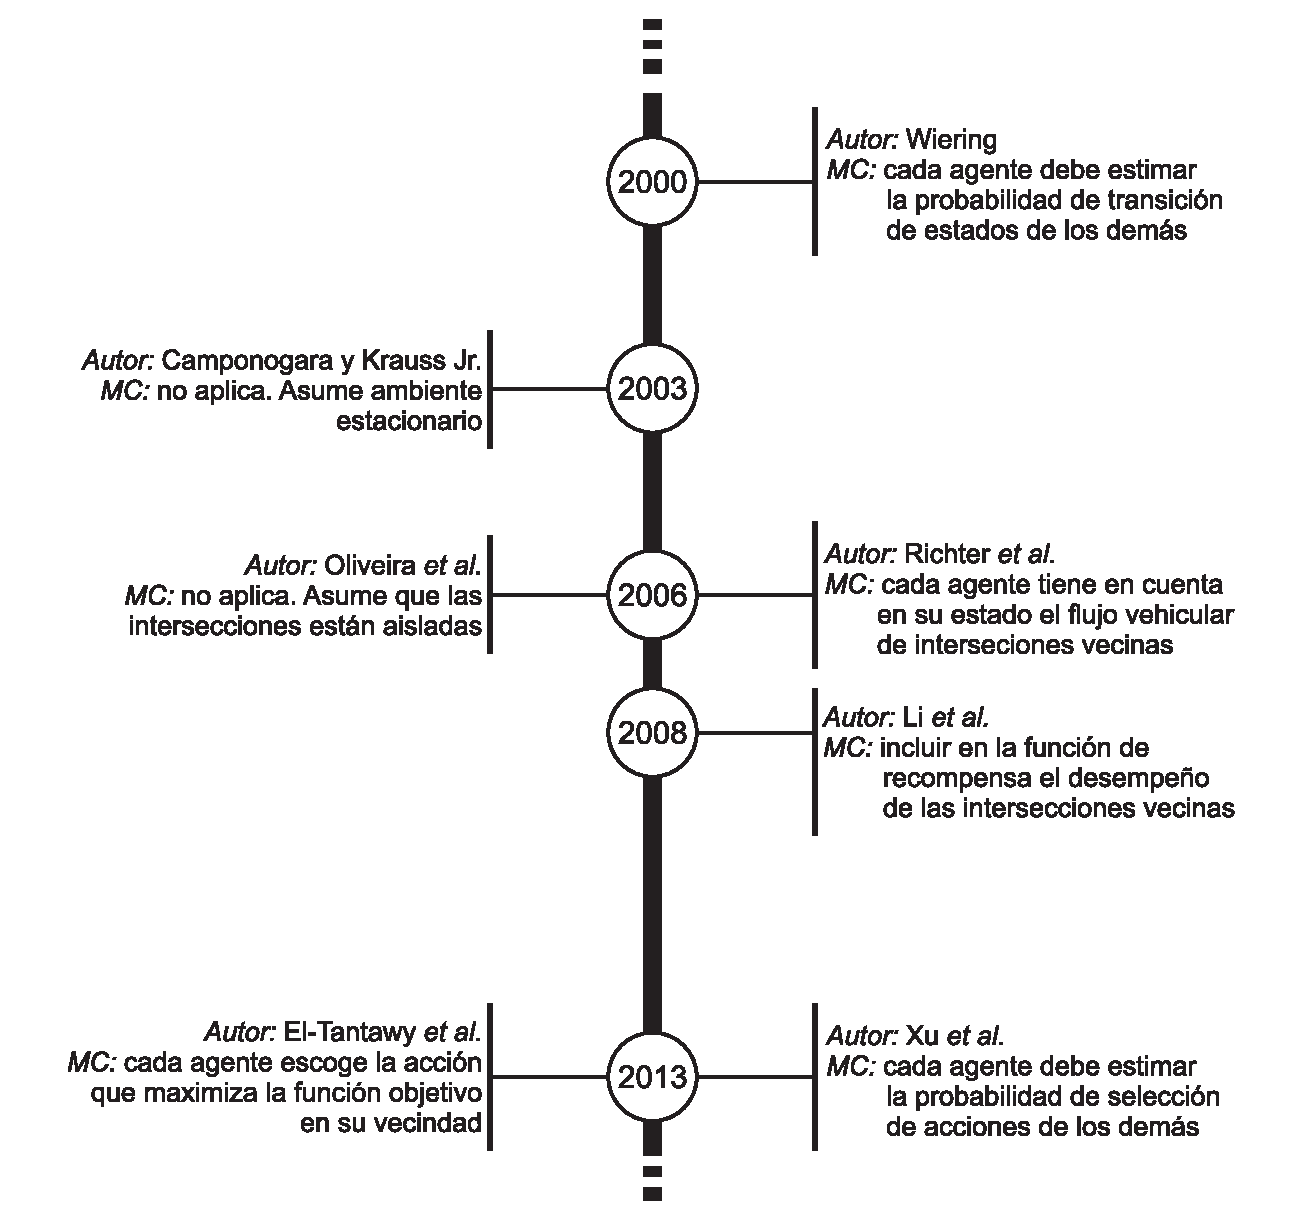
\includegraphics[scale=0.4]{./graficas/estArt2.eps}
\end{center}
\end{frame}

\end{document}
